\documentclass[UTF8,a4paper,zihao=5,fontset=fandol]{ctexart}

\usepackage{geometry}
\usepackage{graphicx}
\usepackage{float}
\usepackage{booktabs}
\usepackage{array}
\usepackage{xcolor}
\usepackage{listings}
\usepackage{caption}
\usepackage{needspace}

\geometry{top=2.2cm,bottom=2.0cm,left=2.6cm,right=2.4cm}
\pagestyle{empty}
\raggedbottom
\setlength{\parindent}{2em}
\setlength{\parskip}{0.2em}
\linespread{1.12}

\captionsetup{font=small,labelfont=bf,labelsep=space}

\definecolor{codebg}{RGB}{248,248,248}
\definecolor{commentgreen}{RGB}{0,120,0}

\lstdefinestyle{cstyle}{
    language=C,
    basicstyle=\ttfamily\small,
    keywordstyle=\color{blue}\bfseries,
    commentstyle=\color{commentgreen},
    stringstyle=\color{red!60!black},
    numbers=left,
    numberstyle=\tiny\color{gray},
    frame=single,
    backgroundcolor=\color{codebg},
    breaklines=true,
    columns=fullflexible,
    tabsize=4,
    showstringspaces=false
}

\newcommand{\sectiontitle}[1]{%
    \vspace{0.7em}
    \noindent{\zihao{-4}\heiti #1}\par
    \vspace{0.25em}
}

\newcommand{\reportfig}[3]{%
    \begin{figure}[H]
        \centering
        \includegraphics[width=#1\textwidth]{figures/#2}
        \caption{#3}
    \end{figure}
}

\newcommand{\twopics}[4]{%
    \begin{figure}[H]
        \centering
        \begin{minipage}[t]{0.48\textwidth}
            \centering
            \includegraphics[width=\textwidth]{figures/#1}
            \caption{#2}
        \end{minipage}
        \hfill
        \begin{minipage}[t]{0.48\textwidth}
            \centering
            \includegraphics[width=\textwidth]{figures/#3}
            \caption{#4}
        \end{minipage}
    \end{figure}
}

\begin{document}

\begin{center}
    \vspace*{0.8cm}
    {\zihao{2}\songti 电子科技大学\ \underline{\makebox[3.0cm][c]{}}\ 学院\par}
    \vspace{2.0cm}
    {\zihao{1}\heiti 实\ 验\ 报\ 告\par}
    \vspace{1.6cm}
    \begin{minipage}{9.8cm}
        {\zihao{4}\heiti
        课程名称\quad \underline{\makebox[6.8cm][l]{C语言程序设计}}\par
        实验题目\quad \underline{\makebox[6.8cm][l]{中外古籍二手书管理系统}}\par
        提交时间\quad \underline{\makebox[6.8cm][l]{}}\par
        姓\quad\quad 名\quad \underline{\makebox[6.8cm][l]{}}\par
        学\quad\quad 号\quad \underline{\makebox[6.8cm][l]{}}\par}
    \end{minipage}
\end{center}

\vspace{1.0cm}

\sectiontitle{1、需求分析}

本实验设计并实现一个面向中外古籍二手书管理的命令行系统。系统管理对象不是普通新书库存，而是带有收录来源、年代、品相和架位信息的古籍或旧藏书籍。每条古籍记录需要保存编号、书名、作者、国别或地区、类别、年代、品相、收录日期、来源、架位号、价格、库存数量和已售数量。编号在系统中作为唯一标识，用于查询、修改、删除、销售和进货等操作。

从功能上看，系统需要完成古籍信息的录入、浏览、查询、修改和删除，同时能够处理库存变化和销售记录。查询功能应覆盖编号、书名关键词、作者、类别、国别、收录日期、来源和架位号等常用检索条件。库存管理要求销售时检查库存是否充足，进货时能及时更新库存。统计功能需要给出古籍种类数、库存总量、库存估值、总销量、估算销售总额、销量最高古籍、库存最低古籍、低库存预警以及按来源、类别的数量统计。

系统采用文本文件保存数据，程序启动时从文件读取初始古籍信息，退出前或手动保存时将链表中的数据重新写回文件。数据文件使用竖线分隔字段，便于保存中文、英文和带空格的书名、作者信息。整个程序使用纯 C 语言实现，重点体现结构体、指针、链表、文件读写、字符串处理、排序和统计等课程内容。

\sectiontitle{2、方案设计}

系统采用单向链表作为内存中的主要数据结构。链表节点由 \texttt{Book} 结构体表示，节点之间通过 \texttt{next} 指针连接。链表适合本项目的原因是古籍记录数量会随添加、删除而变化，动态申请和释放节点更灵活，也能直接体现 C 语言中指针和动态内存管理的使用。

项目文件按功能分成四类。主程序文件 \texttt{main.c} 负责显示菜单和调度功能；\texttt{book.c} 和 \texttt{book.h} 负责古籍链表的增删改查、销售、进货、排序和统计；\texttt{fileio.c} 和 \texttt{fileio.h} 负责读取、保存古籍数据和追加销售日志；\texttt{utils.c} 和 \texttt{utils.h} 封装输入读取、数字转换、日期校验、字符串处理等通用函数。这样处理后，主函数只保留系统入口和菜单控制，具体业务逻辑分布在对应模块中，程序结构比较清楚。

数据文件位于 \texttt{data/books.txt}，每行一条记录，字段顺序固定为：

\Needspace{6\baselineskip}
\begin{lstlisting}[style=cstyle]
id|title|author|country|category|period|condition|collectionDate|source|shelfCode|price|stock|sold
\end{lstlisting}

系统运行流程可以概括为：启动时读取文件并建立链表；用户通过菜单选择功能；所有业务操作直接修改链表；保存时遍历链表并写回文件；退出前释放链表节点。查询和统计均通过链表遍历完成，排序采用链表冒泡排序并交换节点数据。由于课程项目数据规模不大，该方法实现直观，便于调试和说明。

\sectiontitle{3、程序实现}

程序的核心结构体如下。字符串字段采用固定长度字符数组保存，价格使用 \texttt{double}，库存和销量使用 \texttt{int}，最后的 \texttt{next} 指针用于连接下一个节点。

\Needspace{18\baselineskip}
\begin{lstlisting}[style=cstyle]
typedef struct Book {
    char id[20];
    char title[80];
    char author[50];
    char country[30];
    char category[30];
    char period[30];
    char condition[30];
    char collectionDate[20];
    char source[50];
    char shelfCode[30];
    double price;
    int stock;
    int sold;
    struct Book *next;
} Book;
\end{lstlisting}

添加古籍时，程序先申请新节点，再依次输入各个字段。编号输入后会调用 \texttt{isIdExists()} 检查是否重复；价格必须大于 0，库存和已售数量不能为负数；日期必须符合 \texttt{YYYY-MM-DD} 格式。删除古籍时使用前驱指针和当前指针共同遍历链表，能够正确处理删除头节点、中间节点和尾节点的情况。

销售管理是库存变化中最重要的操作。程序根据编号找到目标古籍后，先判断销售数量是否大于库存。库存充足时，库存减少、已售数量增加，并计算本次销售金额；库存不足时直接提示失败，不修改原有数据。

\Needspace{8\baselineskip}
\begin{lstlisting}[style=cstyle]
if (quantity > book->stock) {
    printf("销售失败：库存不足。当前库存为 %d。\n", book->stock);
    return;
}

book->stock -= quantity;
book->sold += quantity;
amount = book->price * quantity;
\end{lstlisting}

文件保存函数遍历链表，将每个节点按固定顺序写入文本文件。读取文件时，程序按竖线拆分字段，并对字段数量、日期、价格、库存、销量和编号重复进行检查。这样既能保证文件格式清楚，也能减少错误数据进入链表。

\Needspace{9\baselineskip}
\begin{lstlisting}[style=cstyle]
fprintf(fp, "%s|%s|%s|%s|%s|%s|%s|%s|%s|%s|%.2f|%d|%d\n",
        p->id, p->title, p->author, p->country, p->category,
        p->period, p->condition, p->collectionDate, p->source,
        p->shelfCode, p->price, p->stock, p->sold);
\end{lstlisting}

输入处理统一使用 \texttt{fgets()} 读取整行，再进行字符串修剪和数值转换，避免直接使用 \texttt{scanf()} 时常见的换行符残留问题。程序退出前调用 \texttt{freeList()} 释放链表节点，减少动态内存长期占用。

\sectiontitle{4、测试结果}

本次测试在 MacBook 本地终端中运行程序，截图均来自实际运行过程。程序启动后能够自动读取 \texttt{data/books.txt}，初始读取 12 条古籍记录，并显示主菜单。浏览全部古籍时，系统以表格形式输出编号、书名、作者、国别、类别、年代、品相、收录日期、来源、架位、价格、库存和已售数量。

\reportfig{0.72}{menu_load.png}{程序启动、读取文件并显示主菜单}
\reportfig{1.0}{display_all.png}{浏览全部古籍信息}

添加功能测试中，系统能够检查重复编号。输入已经存在的 B013 后，程序提示编号已存在，并要求重新输入；随后输入 B014 的完整信息，系统成功添加该古籍。查询功能测试中，按编号查询 B001 可以显示《史记》的完整信息；按书名关键词 The 查询，可以查到 The Republic 和 The Divine Comedy，说明精确查询和关键词查询均能正常工作。

\twopics{add_duplicate.png}{添加古籍与重复编号检查}{search_id.png}{按编号查询 B001}
\reportfig{1.0}{search_title.png}{按书名关键词查询}

修改功能根据编号定位记录。测试中选择 B013，先显示修改前信息，再分别修改价格和库存字段，系统均提示字段修改完成。删除功能测试中，输入 B014 后系统先显示待删除记录，并在确认后删除，避免误删。

\begin{figure}[H]
    \centering
    \begin{minipage}[t]{0.32\textwidth}
        \centering
        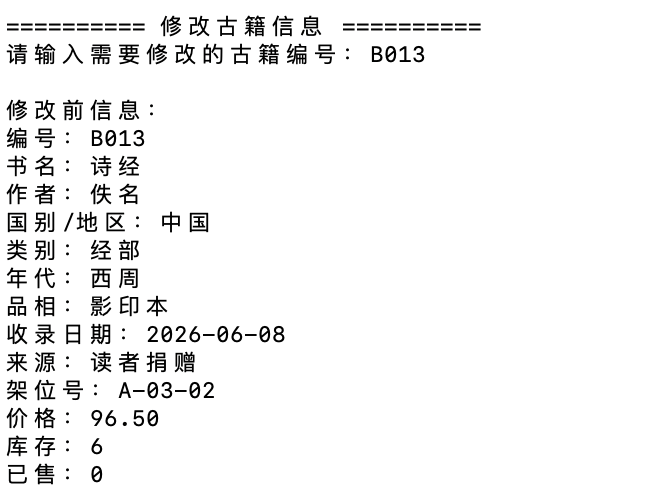
\includegraphics[width=\textwidth]{figures/modify_before.png}
        \caption{显示 B013 修改前信息}
    \end{minipage}
    \hfill
    \begin{minipage}[t]{0.32\textwidth}
        \centering
        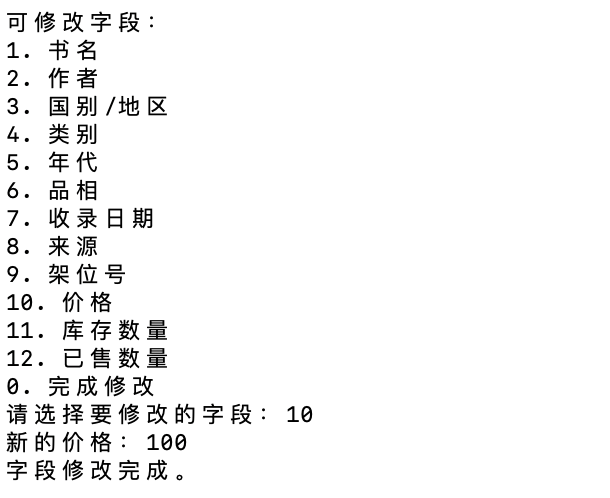
\includegraphics[width=\textwidth]{figures/modify_price.png}
        \caption{修改 B013 价格}
    \end{minipage}
    \hfill
    \begin{minipage}[t]{0.32\textwidth}
        \centering
        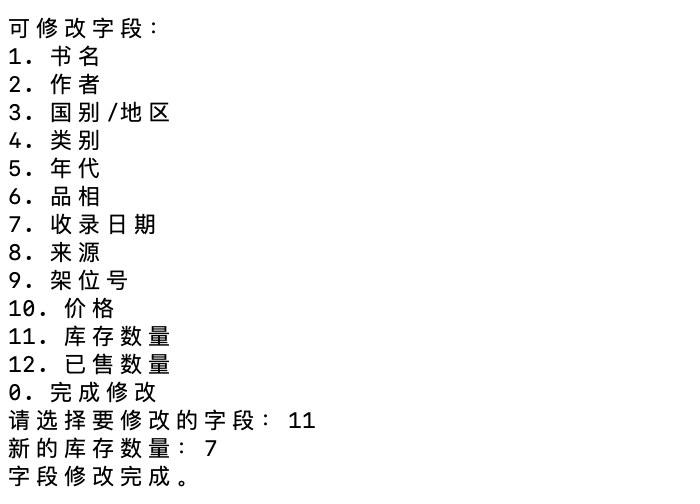
\includegraphics[width=\textwidth]{figures/modify_stock.png}
        \caption{修改 B013 库存}
    \end{minipage}
\end{figure}

\reportfig{0.62}{delete_confirm.png}{删除 B014 前显示记录并确认}

销售和进货功能测试覆盖了成功和失败两种情况。销售 B013 两本时，系统计算本次销售金额 200.00，并将库存更新为 5、已售数量更新为 2。随后尝试销售 B009 十本，由于库存不足，系统提示失败并保持数据不变。进货测试中给 B009 增加 5 本库存，系统显示当前库存更新为 6。

\twopics{sell_success.png}{销售 B013 两本成功}{sell_fail.png}{库存不足时销售失败}
\reportfig{0.56}{purchase.png}{进货 B009 后库存增加}

排序功能测试选择按价格升序排列。输出结果中，价格最低的 Meditations 排在前面，价格最高的《道德经》排在后面，说明排序结果符合预期。统计功能输出古籍种类总数、总库存数量、总库存估值、总销量、估算销售总额、销量最高古籍和库存最低古籍，并进一步按来源和类别统计数量。

\reportfig{1.0}{sort_price.png}{按价格升序排序}
\twopics{statistics_summary.png}{综合统计结果}{statistics_group.png}{按来源和类别统计}

低库存预警功能筛选库存小于等于 3 的记录，测试结果显示 The Divine Comedy、几何原本和资治通鉴等低库存古籍，便于后续补货。保存功能测试中，选择手动保存后，系统提示已保存 13 条古籍记录到 \texttt{data/books.txt}。此外，自动化测试脚本还覆盖了按日期查询新收录古籍和保存后再次读取数据的流程，测试输出文件可用于复核。

\reportfig{1.0}{low_stock.png}{低库存预警}
\reportfig{0.68}{save_file.png}{手动保存数据}

从测试结果看，系统能够完成预期的添加、浏览、查询、修改、删除、销售、进货、排序、统计和文件保存功能。非法输入和边界情况也有基本处理，例如重复编号、库存不足和删除确认等。由于终端对中英文字符宽度的处理不同，表格列宽在不同系统中可能略有差异，但各字段内容能够正常显示，不影响功能判断。

\sectiontitle{5、实验心得}

本次实验把 C 语言中的多个基础知识点放在同一个较完整的系统中使用。单独学习结构体、指针或文件读写时，每个知识点都比较独立；真正写成一个信息管理系统后，链表节点的创建、插入、删除、遍历、保存和释放会自然联系在一起，程序也更容易暴露输入处理、边界条件和文件路径等问题。

在实现过程中，链表删除和文件读写是需要特别注意的部分。删除节点时如果没有处理头节点，容易导致链表头丢失；读取文件时如果字段数量不一致，也可能造成数据错位。为了解决这些问题，程序在读取文件时检查字段数量和编号重复，在删除前显示目标记录并要求确认，在退出前释放链表内存。输入部分统一使用整行读取和转换，也让菜单交互比直接使用 \texttt{scanf()} 更稳定。

通过本项目，可以体会到模块化设计对程序可读性的帮助。将菜单调度、古籍业务、文件读写和工具函数分开后，每个源文件的职责比较明确，后续修改某个功能时不需要在一个很长的主函数中查找。系统仍有可以改进的地方，例如销售日志查询、分页显示、按价格区间查询和更严格的编号格式校验等，但作为 C 语言课程综合实验，当前实现已经覆盖了链表、文件、查找、排序、统计和命令行交互的主要训练目标。

\subsection*{GitHub 开源声明}

本项目为 C 语言程序设计课程综合实验项目，主要用于学习结构体、链表、文件读写、模块化程序设计与命令行交互系统的实现方法。项目代码计划开源至 GitHub，仓库地址如下：

GitHub 仓库地址：\underline{\makebox[7cm][c]{}}

本项目仅用于课程学习与个人编程能力训练，不涉及真实商业古籍交易数据。

\end{document}
